\documentclass{article}
\usepackage[utf8]{inputenc}
\usepackage[english,ngerman]{babel}
%% ========================================================================
%%%% MISC usepackages
%% ========================================================================

%% Chemistry
\usepackage{chemfig,chemmacros}
\chemsetup{modules = all}
\chemsetup[redox]{explicit-sign = true}
\chemsetup[phases]{pos=sub}
%\chemsetup[reactions]{before-tag = {R}, tag-open = [, tag-close = ]}
  
%% Maths
\usepackage{amsmath,amssymb,amsthm,textcomp}

%% Physics
\usepackage{siunitx}

%% Graphics
\usepackage{graphicx}
\usepackage{tikz}
\usepackage{rotating}
%\usepackage{subfig}

%% Tables and Lists
\usepackage{enumerate}
\usepackage{multicol}
\usepackage{geometry}
\usepackage{tabu}
\usepackage{listings}
\usepackage{tabularx}

%% Structures and Style
\usepackage{caption}
\usepackage{subcaption}
\usepackage{booktabs}
\usepackage{colortbl}

\usepackage{xcolor}
\usepackage{xfrac}
\usepackage[export]{adjustbox}[2011/08/13]

\usepackage{booktabs}
\usepackage{float}

\usepackage{fancyhdr}

%% Citing and Settings
\usepackage[backend=biber,
style=numeric,
backref=true, 
natbib=true, %% offering natbib-compatible commands
hyperref=true, %% using hyperref-package references
sorting= none,
doi=true,
maxcitenames=10,
maxbibnames=100,
citestyle=numeric
]{biblatex}

\addbibresource{references.bib}

\usepackage[toc,automake]{glossaries}
\include{abbrevations}
\makeglossaries

\usepackage[colorlinks=true,linkcolor=blue]{hyperref}

%% Figure settings
\renewcommand{\figurename}{Abbildung}
\renewcommand{\tablename}{Tabelle}
\renewcommand{\listfigurename}{Abbildungsverzeichnis}
\renewcommand{\listtablename}{Tabellenverzeichnis}

%% ========================================================================
%%%% Document Information
%% ========================================================================

%% Title
\title{Darstellung eines Esters und Aufarbeitung von Bleiabfällen \cite{Versuchsvorschrift}} % Title
\author{Autor: Florian \textsc{Kluibenschedl}} % Author name
\date{Bericht verfasst am: \today} % Date for the report

% Page style - headers
\pagestyle{fancy}
\fancyhf{}
\rhead{PR Allgemeine Chemie A - SS2019}
\lhead{Institut für Allgemeine Chemie - Universität Innsbruck}
\rfoot{Experiment 8 - Seite \thepage}

\begin{document}
  \renewtagform{reaction}[Rgl. ]{}{}
  
  \maketitle % Insert the title, author and date
  
  \begin{center}
    \begin{tabular}{r p{4cm}}
      Versuchsdurchführung am: & 14. März 2019\\ % Date the experiment was performed
      Gruppe, Matrikelnummer: & 3, 11805747 \\
      Lehrveranstaltung: & PR Allgemeine Chemie A \\
      Institut: & Allgemeine, Anorganische und Theoretische Chemie \\
      Assistent: & Viertl Wolfgang % Instructor/supervisor
    \end{tabular}
  \end{center}


  \begin{abstract}
    Da sich die Chemie mit den Eigenschaften von Stoffen beschäftigt, ist es oft notwendig, Stoffe künstlich herzustellen. Die Kenntnis diverser Synthesetechniken ist demnach von großer Bedeutung. 
    
    Im Folgenden wird die säurekatalysierte Synthese eines Essigsäurepentylesters ausgehend von Essigsäure und Pentan-1-ol beschrieben. Bei der praktischen Durchführung konnte eine Ausbeute von $\approx \SI[mode=text]{64}{\percent}$ erzielt werden. Der Ester war unlöslich in Wasser und verdünnter Essigsäure (1:9 - V/V) aber löslich in konz. Essigsäure und Pentan-1-ol. Die Brennprobe zeigte eine mittelmäßige Rußentwicklung. Außerdem roch die erhaltene Lösung stark nach Birne.\\
    
    Im zweiten Teil wurden Bleiabfälle aus Aufgabe 3 aufgearbeitet, da eine gesättigte \ch{PbI2} Lösung nicht den zulässigen Grenzwert an \ch{Pb\pch[2]\aq} einhält. Dazu wurde eine Umfällung mit \ch{Na2S} zum schwerer löslichen \ch{PbS} durchgeführt. Die erhaltene Lösung konnte ohne Bedenken in den Abfluss geleert werden. 
    
  \end{abstract}
  
  \pagebreak 
  
  \section{Darstellung eines Esters}
  
    \subsection{Theoretische Grundlagen}
  
      \subsubsection{Motivation} \label{sec:Motivation}
  
        Ester stellen eine wichtige organische Stoffgruppe dar und kommen in vielen Bereichen zum Einsatz. So sind sie beispielsweise in Aromastoffen, Weichmachern oder Insektiziden enthalten \cite{EsterEigenschaften}. Der in diesem Versuch synthetisierte Essigsäurepentylester findet vor allem Verwendung als Lösungsmittel in der Lackindustrie und der Chromatographie und riecht nach Birne \cite{Essigsaurepentyl}. Die Darstellung erfolgt über säurekatalysierte Veresterung von Pentan-1-ol\footnote{im Folgenden wird der besseren Lesbarkeit wegen Pentan-1-ol mit Pentanol bezeichnet} mit Essigsäure - siehe \ref{fig:EssigsaureReaktion}. 
        
        \begin{figure}[h]
          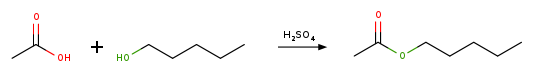
\includegraphics[scale=0.55, center]{Graphiken/Reaktionen/ReactionEsters.png} 
          \caption[Reaktionsgleichung der Darstellung des Essigsäurepentylesters, Quelle: Autor]{Reaktionsgleichung der Darstellung des Essigsäurepentylesters. Anm.: \ch{H2O} entsteht als weiteres Reaktionsprodukt}
          \label{fig:EssigsaureReaktion}
        \end{figure}
        
        Als Katalysatoren eignen sich Säuren mit schwachen Nukleophilen als Anionen, weswegen in diesem Experiment Schwefelsäure verwendet wurde. Der zugehörige Mechanismus wird im Folgenden beschrieben.
        
        \begin{figure}[h]
          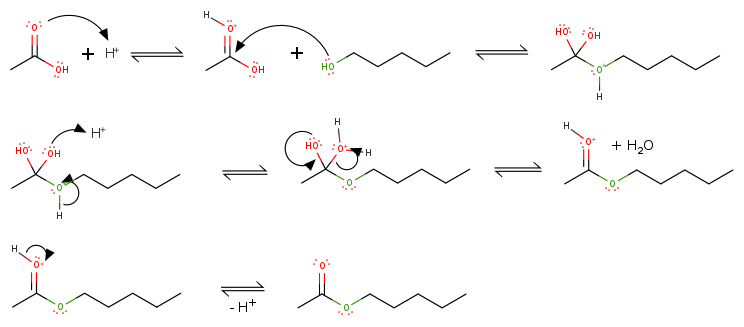
\includegraphics[scale=0.55, center]{Graphiken/Reaktionen/MechanismVeresterung.png} 
          \caption[Reaktionsgleichung Mechanismus der Veresterung, Quelle: Autor]{Mechanismus der säurekatalysierten Veresterung \cite[S. 208]{Clayden}}
          \label{fig:Mechanismus}
        \end{figure}
        
        Im ersten Schritt wird das O-Atom der Carbonsäuregruppe protoniert. Es folgt ein nukleophiler Angriff des O-Atoms des Alkohols an das elektrophile C-Atom der Carbonsäuregruppe. Im nächsten Schritt wird das H-Atom des O-Atom vom Alkohol (grün) abgespalten und geht formal an ein O-Atom der ehemaligen Carbonsäuregruppe (rot). Es folgt die Abspaltung von \ch{H2O} und \ch{H\pch}. 
        
      \subsubsection{Ziel des Experiments}
    
        Auf Basis der obigen Überlegungen ist das Ziel, einen Essigsäurepentylester mit möglichst goßer Ausbeute zu synthetisieren. Außerdem sollen bestimmte Eigenschaften des Esters wie Löslichkeit, Geruch und Brennbarkeit bestimmt bzw. überprüft werden. 
    
    \subsection{Experimenteller Teil}
  
      \subsubsection{Verwendete Materialien}
              
        \begin{table}[H]
          \centering
          \caption[Materialienliste Estersynthese, Quelle: Autor]{Auflistung der verwendeten Geräte und Chemikalien}
          \label{tab:Materialien}
        
          \begin{tabular}{@{}ll|p{4.5cm}l@{}}
            \toprule
              Geräte & Hersteller & Chemikalie & Hersteller \\ \midrule
              \SI[mode=text]{100}{\milli\litre} Rundkolben & DURAN & konz. \ch{H2SO4} - \SI[mode=text]{96}{\percent} (w/w), $\rho = \SI[mode=text]{1.84}{\gram\per\milli\liter}$ & Vorrat \\
              Magnetrührer & CAT M 6.1 & Pentanol & Vorrat \\
              \SI[mode=text,separate-uncertainty]{50}{\milli\litre} Messzylinder & BRAND & deionisiertes \ch{H2O} & Labor \\
              Rührfische &  & Essigsäure &  \\
              Dimrothkühler inkl. Kühlschläuche &  &  &  \\
              Stativ mit Klammern &  &  &  \\
              2 Universalklammern &  &  &  \\ 
              Heizpilz &  &  &  \\
              Glasrichter &  &  &  \\
              Faltenfilter &  &  &  \\
              \SI[mode=text]{600}{\milli\liter} Scheidetrichter &  &  &  \\ 
              \SI[mode=text]{100}{\milli\liter} Becherglas & DURAN &  &  \\ 
              Universalindikator-Papier &  &  &  \\ \bottomrule
          \end{tabular}
        \end{table}
    
    \pagebreak
    
      \subsubsection{Versuchsdurchführung} \label{sec:Versuch}
    
        \begin{figure}[h]
          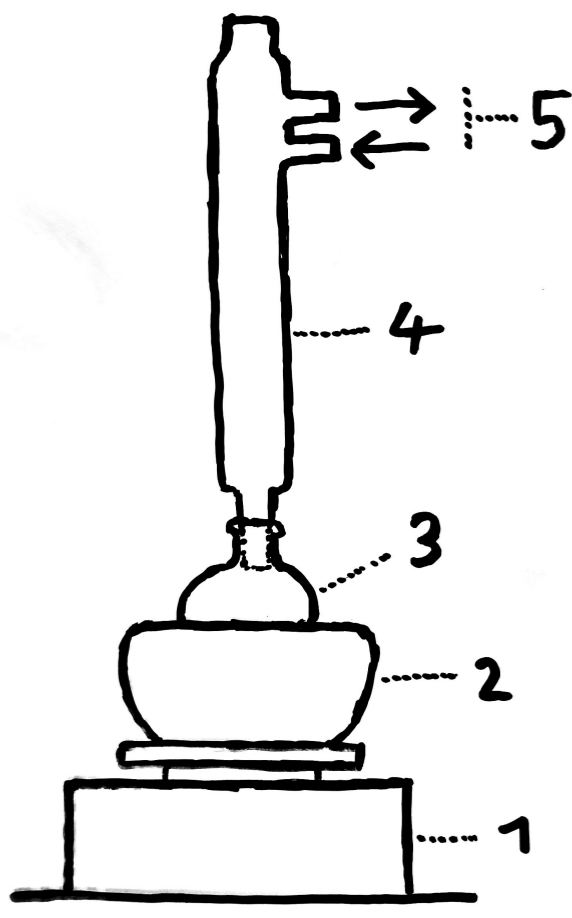
\includegraphics[scale=0.3, center]{Graphiken/Versuchsanordnungen/VersuchsanordnungSynthese.png} 
          \caption[schematische Versuchsanordnung Estersynthese, Quelle: Autor]{schematische Versuchsanordnung: (1) Magnetrührer, (2) Heizpilz, (3) \SI[mode=text]{100}{\milli\litre} Rundkolben, (4) Dimrothkühler, (5) Anschluss der Kühlschläuche inkl. Angabe der Flussrichtung}
          \label{fig:Versuchsanordnung}
        \end{figure}
        
        Die Apparatur wurde wie in Abbildung \ref{fig:Versuchsanordnung} dargestellt aufgebaut. Dabei wurde insbesondere darauf geachtet, Spannungen zwischen den Glasgeräten zu vermeiden. Die Schliffe  wurden gefettet. Die Kühlschläuche wurden wie gezeigt angeschlossen und vor der Befestigung des Kühlers auf Dichtheit überprüft. Rundkolben und Rückflusskühler wurden über Klammern an einem Stativ befestigt. In je einem \SI[mode=text,separate-uncertainty]{50}{\milli\litre} Messzylinder wurden \SI[mode=text]{25}{\milli\liter} konz. Essigsäure und \SI[mode=text]{15}{\milli\liter} Pentanol vorgelegt. \SI[mode=text]{1}{\milli\liter} konz. \ch{H2SO4} wurden in einem \SI[mode=text]{10}{\milli\liter} Messzylinder bereitgehalten. Die drei Reagienzen wurden in den Rundkolben überführt, ein Rührfisch zugegeben und der Rückflusskühler aufgesetzt. Anschließend wurde mit dem Heizpilz auf Stufe 2 für ca. \SI[mode=text]{45}{\minute} unter Rückfluss gekocht. Um den Abkühlvorgang nach dem Kochen zu beschleunigen, wurde der Heizpilz vorsichtig entfernt. Nach ca. \SI[mode=text]{7}{\minute} abkühlen an der Luft wurde der Kolben in ein Eisbad getaucht und der Rührfisch entfernt. Der Kolbenschliff wurde mit einem Papiertuch entfettet, um einen Verlust an Produkt zu vermeiden.
        
        Um das Produkt aufzuarbeiten, wurde die nun kalte Lösung im Rundkolben in einen \SI[mode=text]{600}{\milli\liter} Scheidetrichter transferiert. Es wurde zweimal mit \SI[mode=text]{100}{\milli\liter} deionisiertem Wasser extrahiert. Die leichtere wässrige Phase wurde beide Male verworfen. In einem \SI[mode=text]{100}{\milli\liter} Becherglas wurde die organische Phase mit \ch{Na2SO4} als Trocknungsmittel versetzt, bis der \textit{Schneegestöber-Effekt} einsetzte. In einem Faltenfilter wurde das feste \ch{Na2SO4} abfiltriert, wobei die nun wasserfreie organische Phase im gereinigten \SI[mode=text]{50}{\milli\liter} Messzylinder gesammelt wurde. Die erhaltene Lösung sollte nun wasserfrei sein und im Idealfall ausschließlich den Essigsäurepentylester enthalten. Die Volumen im Messzylinder entspricht der protokollierten Ausbeute. 
        
        Im Anschluss wurde die Löslichkeit in Wasser, konz. Essigsäure, verdünnter Essigsäure - 1:9 (V/V) und Pentanol getestet. Auch der \pH-Wert wurde mithilfe eines Universalindikator-Papiers bestimmt. 
         
      \subsubsection{Auswertung} \label{sec:AuswertungSynthese}
    
        Um die theoretische Ausbeute zu berechnen, muss der limitierende Faktor in der Reaktion berechnet werden. Dazu wird die Stoffmenge an eingesetzter Essigsäure mit jener von Pentanol verglichen. Diese errechnen sich wie unten dargestellt.
        
        \begin{equation}
          n_{\ch{CH3COOH}} = \frac{\rho_{\ch{CH3COOH}} * V_{\ch{CH3COOH}}}{M_{\ch{CH3COOH}}} = \frac{1.05 * 25}{60.05} = \SI[mode=text]{0.44}{\mole}   
        \end{equation}
        
        \begin{equation}
          n_{Pentanol} = \frac{\rho_{Pentanol} * V_{Pentanol}}{M_{Pentanol}} = \frac{0.81 * 15}{88.15} = \SI[mode=text]{0.14}{\mole}   
        \end{equation}
        
        Wie man sieht, ist der limitierende Faktor die Stoffmenge an Pentanol $\Rightarrow n_{Ester} = n_{Pentanol}$, da die Stöchiometrie der Reaktion 1:1 ist. Die theoretische Ausbeute kann nun wie folgt berechnet werden.
        
        \begin{equation}
          m_{Ester} = n_{Ester} * M_{Ester} = \SI[mode=text]{17.9}{\gram} \Rightarrow V_{Ester} = \frac{m_{Ester}}{\rho_{Ester}} \approx \SI[mode=text]{20.4}{\milli\liter}
        \end{equation}
      
      \subsubsection{Literaturwerte}
    
        In Tabelle \ref{tab:Messdaten} sind die Dichten angeführt, die für die Auswertung des Versuchs wie in  \ref{sec:AuswertungSynthese} beschrieben, benötigt werden. Sie wurden der Versuchsvorschrift entnommen. \citep{Versuchsvorschrift}.
      
        \begin{table}[H]
          \centering
          \caption[Mess- und Literaturdaten, Quelle: Autor]{Mess- und Literaturdaten}
          \label{tab:Messdaten}
          \begin{tabular}{@{}ll@{}}
            \toprule
              & Wert \\ \midrule
             $\rho_{\ch{CH3COOH}}$ & \SI[mode=text]{1.05}{\gram\per\milli\liter} \\
             $\rho_{Pentanol}$ & \SI[mode=text]{0.81}{\gram\per\milli\liter} \\
             $\rho_{Ester}$ & \SI[mode=text]{0.88}{\gram\per\milli\liter} \\ \bottomrule
          \end{tabular}
      \end{table}      
     
      Die für die Berechnung benötigten molaren Massen wurden mithilfe der in \ref{sec:Motivation} angegebenen Strukturformeln und einem Periodensystem berechnet. $M_{\ch{CH3COOH}} = \SI[mode=text]{60.05}{\gram\per\mole}$, $M_{Pentanol} = \SI[mode=text]{88.15}{\gram\per\mole}$, $M_{Ester} = \SI[mode=text]{130.19}{\gram\per\mole}$
      
    %\pagebreak     
     
    \subsection{Ergebnisse und Diskussion}
      
      Im \SI[mode=text]{50}{\milli\liter} Messzylinder konnten \SI[mode=text]{13}{\milli\liter} Essigsäurepentylester aufgefangen werden. Die Ausbeute errechnet sich dann als Verhältnis zur in \ref{sec:AuswertungSynthese} berechneten theoretischen Ausbeute zu $\approx \SI[mode=text]{64}{\percent}$. Ein Wert für die Literaturausbeute konnte nicht gefunden werden.  \\
      
      Es wurde beobachtet, dass das Produkt in deionisiertem Wasser und in verdünnter Essigsäure nicht löslich war, jedoch schon in konz. Essigsäure und Pentanol. Mit diesem Ergebnis kann unter anderem auf die Reinheit des Produktes geschlossen werden. Der Essigsäurepentylester ist unpolarer im Vergleich zu Wasser und verdünnter Essigsäure. Eine gute Löslichkeit in diesen Lösungsmitteln würde auf einen hohen Wassergehalt und damit geringe Reinheit hinweisen\footnote{in diesem Fall wäre zu hinterfragen, ob das Produkt überhaupt entstanden ist!}. Um die Reinheit des Produktes genauer zu untersuchen, müssten Dichteuntersuchungen, ... durchgeführt werden. 
      
      Das Indikatorpapier zeigte einen \pH-Wert im neutralen Bereich, was bedeutet, dass die Schwefelsäure bei der Extraktion erfolgreich aus der organischen Phase entfernt werden konnte.
      
      Das Produkt roch stark nach Birne, was einhergeht mit der Tatsache, dass man im Alltag auch vom Birnenester spricht \cite{Essigsaurepentyl}. Die Brennprobe der flüssigen Lösung zeigte eine orange Flamme mit mittelmäßiger Rußentwicklung im Vergleich zu einem Essigsäurebutylester. \\
      
      Zusammenfassend wird die Synthese als gelungen betrachtet. Die Ausbeute kann aufgrund des fehlenden Literaturwerts leider nicht in Relation gesetzt werden. Dennoch konnten die erwarteten Eigenschaften hinsichtlich Löslichkeit, Geruch und Brennbarkeit bestätigt werden. \\
      
      Um die Ausbeute zu erhöhen, kann beispielsweise für längere Zeit unter Rückfluss gekocht werden. Auch könnte man den Extraktionsprozess optimieren, indem man beispielsweise nicht zweimal mit je \SI[mode=text]{100}{\milli\liter} deionisiertem Wasser sondern z. B. viermal mit je \SI[mode=text]{50}{\milli\liter} extrahiert. Gemäß des Nernst'schen Verteilungsgleichgewichtes müsste eine höhere Ausbeute zu erwarten sein.
     
     \pagebreak
     
     \section{Aufarbeitung von Bleiabfällen}
     
       \subsection{Theoretische Grundlagen}
         
         \subsubsection{Motivation}
           
           Blei ist toxisch und mitunter umweltgefährdend \citep{blei}. Deswegen müssen bei der Entsorgung von Bleiabfällen bestimmte Grenzwerte eingehalten werden. Blei(II)iodid ist ein schwerlösliches Salz ($K_{L} = \num{9.8d-9}$ bei \SI[mode=text]{25}{\degreeCelsius} \cite{solubilityConstants}). Die Löslichkeit errechnet sich zu $\SI[mode=text]{1.35d-3}{\mole\per\liter} \equiv \SI[mode=text]{621.5}{\milli\gram\per\liter}$. Der Emmissionsrichtwert für Abwasser beträgt \SI[mode=text]{1.0}{\milli\gram\per\liter} \cite{Versuchsvorschrift}. Damit liegt die Konzentration an Blei in einer gesättigten \ch{PbI2} Lösung über dem Grenzwert, weswegen \ch{PbI2} Abfälle nicht im Abfluss entsorgt werden dürfen. 
           
           Ein Ausweg aus diesem Dilemma ist die Überführung von \ch{PbI2} in noch schwerer lösliches \ch{PbS} ($K_{L} = \num{3.2d-28}$ bei \SI[mode=text]{25}{\degreeCelsius} \cite{solubilityPbS}). Die Löslichkeit von \ch{PbS} errechnet sich zu $\SI[mode=text]{1.8d-14}{\mole\per\liter} \equiv \SI[mode=text]{4.28d-9}{\milli\gram\per\liter}$. Damit wird in einer gesättigten \ch{PbS} Lösung der oben angegeben Grenzwert nicht überschritten, weswegen diese im Abfluss entsorgt werden kann\footnote{natürlich ohne \ch{PbS}, welches im Feststoffabfall entsorgt wird}.
           
           Die Reaktionsgleich für die Umfällung lautet wie folgt.
           
           \begin{reaction}
             PbI2\aq{} + Na2S\aq{} -> PbS\sld{} + 2 NaI\aq{}            
           \end{reaction}
           
           Die oben angegebenen Werte für die jeweilige Löslichkeit können wie in dargestellt berechnet werden. Die Umrechnung in \si{\gram\per\liter} wird nicht explizit angeführt. 
           
           \begin{equation}
             L_{M,\ch{PbI2}} = \sqrt[3]{\frac{K_{L,\ch{PbI2}}}{4}}
           \end{equation}   
           
           \begin{equation}
             L_{M,\ch{PbS}} = \sqrt{K_{L,\ch{PbS}}}
           \end{equation}  
                             
         \subsubsection{Ziel des Experiments}
         
           Das Ziel des Experiments ist die Aufarbeitung von \ch{PbI2} Abfällen durch Umfällung mit \ch{Na2S}.
           
       \subsection{Experimenteller Teil}
       
         \subsubsection{Verwendete Materialien}
              
        \begin{table}[H]
          \centering
          \caption[Materialienliste Aufarbeitung der Bleiabfälle, Quelle: Autor]{Auflistung der verwendeten Geräte und Chemikalien}
          \label{tab:MaterialienAbfall}
        
          \begin{tabular}{@{}ll|ll@{}}
            \toprule
              Geräte & Hersteller & Chemikalie & Hersteller \\ \midrule
              2 \SI[mode=text]{600}{\milli\litre} Becherglas & DURAN & \ch{PbI2} Lösung & Vorrat - aus Aufgabe 3 \\
              Magnetrührer & CAT M 6.1 & festes \ch{Na2S} & Vorrat \\
              Rührfische &  &  &  \\
              Glastrichter mit Faltenfilter &  &  &  \\
              Spatel &  &  &  \\ \bottomrule
          \end{tabular}
        \end{table}
        
        \subsubsection{Versuchsdurchführung}
        
         In einem \SI[mode=text]{600}{\milli\litre} Becherglas wurden ca. \SI[mode=text]{300}{\milli\litre} einer \ch{PbI2} Lösung vorgelegt und mit ca. \SI[mode=text]{8}{\gram} \ch{Na2S} versetzt\footnote{die zugegebene Sulfid-Menge sollte bei weitem ausreichen, fast das gesamte Blei zu fällen}. Bei \SI[mode=text]{200}{rpm} wurde bei \SI[mode=text]{300}{\degreeCelsius} bis zum Sieden erhitzt. Die entstehenden schwarzen Klumpen wurden mit einem Spatel zerstoßen, um etwaige Einschlüsse an \ch{PbI2} zu vermeiden. Nach dem Sieden wurde für weitere \SI[mode=text]{10}{\minute} bei \SI[mode=text]{140}{\degreeCelsius} erhitzt. Der Rührfisch wurde entfernt und die Lösung heiß filtriert. Dabei wurde ein Faltenfilter und Glastrichter verwendet.
         
         Die gefilterte Lösung konnte in den Abfluss geleert werden. Der Filter inkl. \ch{PbS} Rückstand wurde im Feststoffabfall entsorgt. 
         
       \subsection{Ergebnisse und Diskussion}
       
         Ergebnisse im klassischen Sinn gibt es in diesem Fall nicht. In welchem Ausmaß die Fällung tatsächlich erfolgte, lässt sich nicht ganz sicher sagen. Natürlich kann man auf die Gültigkeit des Löslichkeitsprodukts vertrauen. Dennoch kann es durch nicht ideale Reaktionsbedingungen wie z. B. Fremdioneneffekt zur Änderung der Löslichkeit kommen. Da die Löslichkeit wie oben angegeben wirklich klein ist, müsste sich diese jedoch um fast 9 Größenordnungen\footnote{damit der Grenzwert nicht eingehalten wird} ändern, was letztendlich doch unrealistisch ist. 
  \pagebreak
  
  \listofreactions
  \printbibliography[title=Literaturverzeichnis]
  \listoffigures
  \listoftables
  
\end{document}
